%%%%%%%%%%%%%%%%%%%%%%%%%%%%
\documentclass[a4paper,11pt,spanish]{report}
%%%%%%%%%%%%%%%%%%%%%%%%%%%%
% LINE SPACING
\newcommand{\linespacing}{1.5}
\renewcommand{\baselinestretch}{\linespacing}
%%%%%%%%%%%%%%%%%%%%%%%%%%%%
%%%%%%%%%%%%%%%%%%%%%%%%%%%%
%BIBLIOGRAPHY STYLE
\usepackage{natbib}
\bibliographystyle{plain}
% \bibliographystyle{plain} for [1], [2] etc.
%%%%%%%%%%%%%%%%%%%%%%%%%%%%

%%%%%%%%%%%%%%%%%%%%%%%%%%%%
% OTHER FORMATTING/LAYOUT DECLARATIONS
% Graphics
\usepackage{algorithm}
\usepackage[noend]{algpseudocode}
\makeatletter
\def\BState{\State\hskip-\ALG@thistlm}
\makeatother

\usepackage[noend]{algpseudocode}
\usepackage{graphicx,color}
\usepackage[english]{babel}
\selectlanguage{English}
\usepackage[utf8]{inputenc}
\usepackage{listings}
\usepackage{amsmath}
\usepackage{microtype}
\usepackage{enumitem}
%\usepackage{minted}
\usepackage{longtable}
\usepackage{booktabs}
\usepackage{epstopdf}
%\usepackage[british]{babel}
% The left-hand-side should be 40mm.  The top and bottom margins should be
% 25mm deep.  The right hand margin should be 20mm.
\usepackage[a4paper,top=2.5cm,bottom=2.5cm,left=2.7cm,right=2.5cm,headsep=10pt]{geometry}
%\flushbottom
% Pages should be numbered consecutively through the main text.  Page numbers
% should be located centrally at the top of the page.
\usepackage{fancyhdr}
\fancypagestyle{plain}{
	\fancyhf{}
	% Text in header
 	%\lhead{\textit{\today}}
	%
	\cfoot{\thepage}
	\renewcommand{\headrulewidth}{0pt}
}
% Paragraph separation and indents
\pagestyle{plain}
\setlength{\parskip}{\baselineskip}%
\setlength{\parindent}{0pt}
%%%%%%%%%%%%%%%%%%%%%%%%%%%%

%%%%%%%%%%%%%%%%%%%%%%%%%%%%
% HYPER REF
\usepackage[colorlinks,pagebackref,pdfusetitle,urlcolor=black,citecolor=black,linkcolor=black,bookmarksnumbered,plainpages=false]{hyperref}
% For print version, use this instead:
%\usepackage[pdfusetitle,bookmarksnumbered,plainpages=false]{hyperref}
%\usepackage{backref}
%\renewcommand{\backrefpagesname}{Cited on}
%%%%%%%%%%%%%%%%%%%%%%%%%%%%

%%%%%%%%%%%%%%%%%%%%%%%%%%%%
% BEGIN DOCUMENT
\begin{document}
\raggedbottom
%%%%%%%%%%%%%%%%%%%%%%%%%%%%

%%%%%%%%%%%%%%%%%%%%%%%%%%%%
% PREAMBLE: roman page numbering i, ii, iii, ...
\pagenumbering{roman}
%%%%%%%%%%%%%%%%%%%%%%%%%%%%

%%%%%%%%%%%%%%%%%%%%%%%%%%%%
%% TITLE PAGE: The title page should give the following information:
%%	(i) the full title of the thesis and the sub-title if any;
%%	(ii) the full name of the author;
%%	(iii) the qualification aimed for;
%%	(iv) the name of the University of Sussex;
%%	(v) the month and year of submission.
\thispagestyle{empty}
\begin{flushright}
\includegraphics[width=6cm]{figures/LOGO_ESCUELA}
\end{flushright}
\vskip40mm
\begin{center}
% TITLE
\huge\textbf{Development of unsupervised learning transformations through supervised learning methods.}
\vskip2mm
% SUBTITLE (optional)
\LARGE\textit{}
\vskip5mm
% AUTHOR
\Large\textbf{Author: Patricia Cortajarena Sauca}

\Large\textbf{Ponente: Carlos Roberto del Blanco Adán}

\Large\textbf{Tutor: Iñigo Cortajarena Sauca}

\end{center}
\vfill
\begin{flushleft}
\large
% QUALIFICATION
Trabajo Fin de Grado \\
ETSIT UPM 	\\
% DATE OF SUBMISSION
Madrid. January, 2018
\end{flushleft}
%%%%%%%%%%%%%%%%%%%%%%%%%%%%

%%%%%%%%%%%%%%%%%%%%%%%%%%%%
% ABSTRACT
\chapter*{Abstract}
\setcounter{page}{3}

The aim of this project is  


%%%%%%%%%%%%%%%%%%%%%%%%%%%%
% ACKNOWLEDGEMENTS
\chapter*{Acknowledgements}

\renewcommand{\baselinestretch}{\linespacing}
\small\normalsize
% ACKNOWLEDGEMENTS HERE:
%%%%%%%%%%%%%%%%%%%%%%%%%%%%%

%%%%%%%%%%%%%%%%%%%%%%%%%%%%%
% TABLE OF CONTENTS, LISTS OF TABLES & FIGURES
\newpage
\pdfbookmark[0]{Contents}{contents_bookmark}
\tableofcontents
\listoftables
\phantomsection
\addcontentsline{toc}{chapter}{List of Tables}
\listoffigures
\phantomsection
\addcontentsline{toc}{chapter}{List of Figures}
%%%%%%%%%%%%%%%%%%%%%%%%%%%%%

%%%%%%%%%%%%%%%%%%%%%%%%%%%%%
% MAIN THESIS TEXT: arabic page numbering 1, 2, 3, ...
\newpage
\pagenumbering{arabic}
%%%%%%%%%%%%%%%%%%%%%%%%%%%%%

%-----------------------------------------------------
% Chapter: Introduction
%-----------------------------------------------------

\chapter{Introduction}
\label{chap:intro}

Working with large datasets and high-dimensional data in nowadays' problems has encouraged the use of dimensionality reduction algorithms which try to preserve as much information as possible even with a reduced number of features used to describe that same dataset. This means  dimensionality reduction algorithms compute new features based on the original ones. Although the number of new features computed are less than the number of original ones, the reduction's objective is to still represent the same information without significant distortion. Thus, time and memory in huge implementations are saved.

Taking into account that this turns into a difficult task, numerous approaches have been proposed.\\
Although the different approaches try to achieve more or less the same aim, they differ from one another and we can not reassure which would suite for a specific problem or even if the behaviour of the algorithm throws the results we expected or needed.

The first point to take into account is the existence of parametric and non-parametric algorithms, depending on whether the dimensionality reduction can be expressed in terms of parameters or not, which can be conclusive when deciding what algorithm to use.\\
Secondly, in both of them we can find different models proposed depending on what to optimize, yet not everything is going to be preserved as well as in the original dataset, so we need to prioritize some aspects.

So the decision of which of them to implement depends on the previous study of our data, the performance requirements and the later purpose and usage of the reduced data.

The non-parametric algorithms have an important disadvantage: as it is said, they don't have parameters which represent the dimensionality reduction; thus, when a new datapoint is provided we need to compute the whole algorithm again to obtain the datapoint's representation in the lower space, instead of computing only the new data.

We hereby propose the study and research of an implementation which replicates the behaviour of a non-parametric dimensionality reduction algorithm. The main objective is to solve the non-parametric's main disadvantage and make the new algorithm capable of being repeatedly used with new datapoint examples, omiting the need to compute the whole dimensionality reduction algorithm every time.\\
The dimensionality reduction algorithms used to base the research are the ones listed below:
\renewcommand{\labelitemi}{\textendash}
\begin{itemize}
\item PCA (Principal Component Analysis)
\item MDS (Multidimensional Scaling)
\item TSNE (T-Stochastic Neighbour Embedding)
\end{itemize}

To conclude, the document is divided into chapters which resume the main steps of this research. Chapter number \ref{chap:stt} describes the State-of-The-Art. It is followed by chapter \ref{chap:frame}, which details the main development of the implementation. Afterwards, chapter \ref{chap:app} describes the main implementation's applications and the corresponding metrics computed to analyse the algorithm's behaviour. The last chapter (chapter \ref{chap:conc}) comprehends the conclusion and resumes the main ideas acquired.

%-----------------------------------------------------
% Chapter: State of the Art
%-----------------------------------------------------

\chapter{State-of-The-Art}
\label{chap:stt}

The most classical dimensionality reduction techniques are know to be PCA \citep{pca} and MDS \citep{mds}. They preserve the true structure of the data even though they are simple to implement and efficiently computable. They rely on linear models to compute data mining on near lower dimensional spaces. A related linear implementation which is based on random projectations of the data is described in \citep{rproj, rproj2}. Some other well-known techniques are ISOMAP \citep{isomap} and t-SNE \citep{tsne}, but their implementations often require more memory and computational time, yet the complexity of the algorithms is higher. Nevertheless, this algorithms are capable of reducing the number of features in non-linear data, where linear models can not faithfully reprensent the data's structure. ISOMAP computes geodesic distances instead of taking into account only euclidean distances while t-SNE's approach calculates probabilities from euclidean distances.

Neural networks have become an essencial tool in machine learning problems and it is certainly used in dimensionality reduction. The autoencoders \citep{auto2, auto} consist on a neuralnet with decreasing number of neurons per layer and then symmetrically more layers are added with the same corresponding increasing neurons per layer. If the output represents without distorsion the input to the net, the middle layer with the fewest number of neurons corresponds to the reduced description of the data. This is represented in figure \ref{autoencoder}.

\begin{figure}[h]
\centering
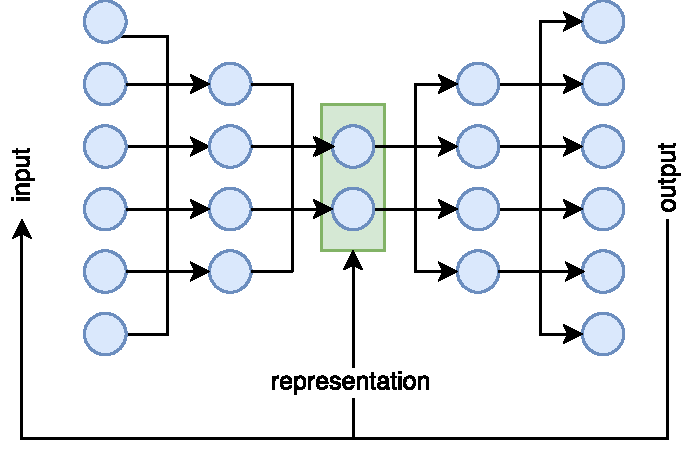
\includegraphics[width=8cm]{figures/autoencoder.pdf}
\caption{\label{autoencoder}Autoencoder neural network.}
\end{figure}

The next sections (sections \ref{sec:pca}, \ref{sec:mds} and \ref{sec:tsne}) resume the main ideas of the algorithms in which the research is based. 

\section{PCA: Principal Component Analysis}
\label{sec:pca}

Principal Component Analysis \citep{pca} algorithm is based on reducing the number of features by processing the correlations between the features of the datapoints. The aim is to eliminate this correlations by transforming the matrix \textbf{X} $\in$ $\Re^{mxn}$ (with m being the number of data points and n de number of features) into an orthogonal basis. By omiting the correlation between columns of the matrix \textbf{X} we are capable of doing away with redundancies.\\
The model starts by computing de covariance matrix, which results in a $\Re^{nxn}$ symmetric matrix. We obtain it by using the next expression:
\begin{center}
cov(\textbf{X}) = $\dfrac{1}{m-1}$ $\textbf{X}^{T}$\textbf{X}
\end{center}
Because the aim of the PCA is to eliminate the correlations, the covariance matrix of the result \textbf{Y} should be a diagonal matrix with just the variances of the columns.\\
PCA is famous because of a great advantage: we can find a linear transformation (\textbf{Y = XP}), which makes this a parametric model, easy to reuse and quite computationally simple.\\
For symmetric matrices (\textbf{X}) we can find eigenvalue decomposition with a diagonal matrix (\textbf{Y}), matching exactly with our linear problem with \textbf{X} and \textbf{Y}.
\begin{center}
\textbf{Y = XP}
$$ cov(\textbf{Y}) = \frac{1}{m-1} \textbf{Y}^{T} \textbf{Y} = \frac{1}{m-1} \textbf{(XP)}^{T} \textbf{XP} = \textbf{P}^{T} cov(\textbf{X})\textbf{P} $$
$$\textbf{D} = \textbf{V}^{T} \textbf{AV}$$
$$ \textbf{A} = cov(\textbf{X}); \textbf{P} = \textbf{V}^{T}; \textbf{D} = cov(\textbf{Y})$$
\end{center}

With the previous expressions we get to the point that, by computing the eigenvectors of the covariance matrix \textbf{X}, we can get a linear transformation from space \textbf{X} to space \textbf{Y}. The eigenvalues matrix obtained (cov(\textbf{Y})) are sorted decreasingly and are the orthogonal basis values. Choosing the \textbf{N} first values of this matrix, being \textbf{N} the desired output dimension, and computing the corresponding eigenvectors, we obtain our reduced dimensionally points, as a basis transformation of our datapoints from the original dataset, by the new basis coordinates.

\section{MDS: Multidimensional Scaling}
\label{sec:mds}

Multidimensional Scaling \citep{mds} in dimensionality reduction tries to create a map which displays the relative distances between the data points. This focuses on getting a lower dimensional map, keeping as much distance information as possible. In case of visualizing data, this dimensional map needs to be a one, two or, at most, three dimensional space.\\
MDS calculates a metric or non-metric solution depending on the data provided, which has to be a \textit{proximity} matrix. This \textit{proximity} matrix quantifies how close the datapoints are. On the one hand for metric solutions, this \textit{proximity} matrix has to be a true distance matrix, while on the other, both dissimilarities or correlations are alternatives to the input for the problem's matrix.

MDS algorithm is based on some ideas explained in the previous section. The \textit{proximity} matrix is always  symmetric and somehow describes the relations between the features, so basically we can treat our problem as a variation of the PCA algorithm.\\
Metric MDS performs the same steps as in PCA, with the modification of being a distance matrix the one computed in this problem.\\
In non metric MDS, we assume a less strict relation and we compute the observed distances as a function of the real distance plus some meassure error. The usable information in this case is going to be the rank order of the previous matrix, which could be the input for the model.\\
The main difference between PCA and MDS is the fact that, because of the need to compute a pairwise distance or proximity matrix, there is no linear transformation that suits both the distance computations plus the matrix operations, so MDS turns to be non-parametric.

\subsection{Stress metric}
\label{ssec:str}

As in every data problem, we need a metric which shows how well the performance given a particular dataset is. In Multidimensional Scaling we compute the \textit{stress} measure that compares the predicted distances with the original ones. Note that obviously this depends on the number of dimensions we want to keep, yet if we lower the number of dimensions, the stress will get higher, because we are representing the same distances relations in a lower dimensional space.
\begin{center}
\( \textit{stress} = \sqrt{\frac{\sum(d_{ij}-d'_{ij})^{2}}{\sum d_{ij}^{2}} } \)
\end{center}
$d_{ij}$ represents the original distance and $d'_{ij}$ is the predicted distance based on the MDS model. This last value is either a predicted true distance or a function which represents the non-metric transformation of the data.\\
Regarding the previous expression, if our prediction stands well for the original data, the stress value should lower, relating zero stress to the perfect performance of the MDS  algorithm. 

\section{TSNE: T-Stochastic Neighbour Embedding}
\label{sec:tsne}

T-Stochastic Neighbour Embedding \citep{tsne} is our non-linear example of dimensionality reduction. It relies on Stochastic Neighbour Embedding (SNE). The main reason why this algorithm is used is because it is capable of representing both the local and the global structure of the original data. As said, this section will be divided in two: the basis SNE and the t-SNE upgrades.

\subsection{SNE}
\label{ssec:sne}

SNE approaches the dimensionality reduction by converting the Euclidean distances into conditional probabilities as a way of expressing similarities between points. That means we measure the similarity of two points $x_{i}$, $x_{j}$ as the probability $p_{i|j}$ of considering the second one as a neighbour of the first. The probability in the original and in the low dimensional space is computated as seen:

$$ p_{i|j} = \frac{exp(-||x_{i}-x_{j}||^{2}/2\sigma_{i}^{2})}{\sum _{k\neq i} exp (-||x_{i}-x_{k}||^{2}/2\sigma_{i}^{2})}$$

$$ q_{i|j} = \frac{exp(-||y_{i}-y_{j}||^{2})}{\sum _{k\neq i} exp (-||y_{i}-y_{k}||^{2})} $$

This expressions represent gaussian distributions centered in each datapoint $x_{i}$, where $\sigma_{i}$ is the example's variance. The conditional probability represents whether the point $x_{j}$ is considered a datapoint's neighbour or not. According to the value of $\sigma_{i}$ the probabilities change, so it is chosen depending on the density of the data. In a dense region, a smaller value of $\sigma_{i}$ is more appropiate than in a sparse region. Having decided which value to use for each of the datapoints, we obtain a probability distribution, $P_{i}$, that is computed as explained in the next paragraph.

As the point of this metric is to compute similarities as probabilities, we can calculate the mismatch between $p_{i|j}$ and $q_{i|j}$ with all the datapoints and consequently obtain the algorithm's behaviour by analysing how many neighbours have been mantained in the low dimensional map. In terms of conditional probabilities, Kullback-Leibler divergence perfectly suits this need. Summing up all the previous ideas we get to the point of minimizing the cost function described as:

$$ C = \sum\limits_{i} KL(P_{i}||Q_{i}) = \sum\limits_{i} \sum\limits_{j} p_{i|j} log \frac{p_{i|j}}{q_{i|j}}$$

The limitations of this algorithm are the non symmetric general expression of the Kullback-Leibler divergence, the difficulty to optimize the cost function, the fact that we need to choose diferent values of the variance depending on the point and the "crowding problem". T-SNE tries to solve this limitations as in the next section is described.

\subsection{t-SNE}
\label{ssec:tsne}

Although SNE is capable of showing good visualizations, t-SNE was proposed as a modified algorithm which tried to make its behaviour more accurate and easy to compute.\\
First of all, instead of minimizing the sum of the different KL divergences along all the datapoints, another way of computing the cost is presented: we are trying to minimize a single KL divergence between a joint probability P and the same in the low dimensional space, Q. With this symmetric aproach, we ommit the need to obtain the variance value for each datapoint and the cost function is much easier to compute and optimize, so does the gradient.

$$ C = KL(P||Q) = \sum\limits_{i} \sum\limits_{j} p_{ij} log \frac{p_{ij}}{q_{ij}}$$

$$ \frac{\partial C}{\partial y_{i}} = 4 \sum\limits_j (p_{ij} - q_{ij}) (y_{i} - y_{j}) $$

Secondly, t-SNE handles with the problem known as "crowding problem" by introducing a heavy-tailed distribution, the Student-t distribution, rather than a Gaussian for the low-dimensional space. The "crowding problem" appears when we want to faithfully represent the mutually equidistant points when reducing from high-dimensional space to low-dimensional space. This task tends to be quite difficult because the area available in a lower space is less than in the higher one. In the end, the points tend to crush together in the center of the map, so the result is the impossibility of representing the true distances from the original dataset.\\
The t-Student distribution is considered a heavy-tailed distribution because it allows to represent a moderate distance as a much larger distance in the map without any inconvenience.
Therefore, the joint probabilities are now then computed as follows:

$$ q_{ij} = \frac{(1+ ||y_{i}-y_{j}||^2)^{-1}} {\sum\limits_{k\neq l} (1+ ||y_{k}-y_{l}||^2)^{-1} }$$

The reason why this particular distribution was chosen is because it is related to the Gaussian distribution, as the t-Student is an infinite mixture of Gaussians.\\
To conclude, the gradient of the Kullback-Leibler divergence taking into account this changes in the Q low-dimensional space stands for the next expression:

$$ \frac{\partial C}{\partial y_{i}} = 4 \sum\limits_j (p_{ij} - q_{ij}) (y_{i} - y_{j}) (1+ ||y_{i}-y_{j}||^2)^{-1}$$

%\begin{figure}
%\centering
%\includegraphics[width=16cm]{figures/prices.pdf}
%\caption{\label{prices}Box-plot of prices for each neighborhood.}
%\end{figure}

%-----------------------------------------------------
% Chapter: Framework
%-----------------------------------------------------

\chapter{Framework}
\label{chap:frame}

We hereby propose the development of a supervised learning tool which learns the embedding derived by an unsupervised learning method, which could be used in real machine learning applications.

The two main supervised learning algorithms used in today's applications are especially Neural Networks and Decision Trees. To know which of them or even if both could suit our problem we study their main characteristics and differences.\\
First of all, decision trees are known to be faster and easier to train, and their results are very interpretable. On the other hand, neuralnets are slower and less interpretable. Neural networks are prone to overfitting if the size of the given dataset is not large enough or if the parameters learnt are not the best in the algorithm's performance, while decision trees are less prone to overfit if pruned (eliminating the tree's branches which do not contribute  correctly to the classification). What really makes the difference from one another is the fact that neuralnets are capable of having two output values or the number of values required as outputs whether the decision trees only show one output per performance. If we wanted to extract more than one value we would be required to have one diferent tree for each output. That increases computational complexity as the number of output dimensions increase.

Taking into account the characteristics and differences between neuralnets and decision trees, the main supervised learning algorithm tested in our development are neural networks, yet it is a powerful and efficient tool which can learn from easy functions up to complicated non-linear models. The advantage of our framework relies on the fact that, as it's said, due to being a supervised algorithm, it is possible to reuse the parameters learned in the fitting process.

Multidimensional Scaling and T-Stochastic Neighbour Embedding are both non-parametric dimensionality reduction algorithms. As it was explained in the introduction (Chapter \ref{chap:intro}), this algorithms can not be expressed in terms of parameters, so this means once the algorithm is computed, if we want to add a new datapoint to the dataset and then obtain its reduced embedded vector, it would be necessary to compute everything again so that that the total ouput includes the new datapoint's output too. Thus, this means a lot of computational work.

Going in depth into the problem, that means if we have a set of \textbf{m} datapoints with \textbf{n} features each, and we want to represent those points in a two-dimensional space, we look forward to using a neuralnet (supervised algorithm) which learns that embedding from \textbf{n} dimensions into two, replicating any of the previously mentioned dimensionality reduction algorithms (unsupervised non-parametric algorithm).\\ The neural network needs to be trained at least once, so we need to compute the dimensionality reduction algorithm once (step 1, figure \ref{figurenet}) to input the dataset into the neuralnet and set the output as the reduced values just computed. Having the neuralnet trained (step 2, figure \ref{figurenet}), as soon as we get a new datapoint, instead of recalculating the MDS or t-SNE algorithm, we can reuse the neuralnet's parameters to obtain the predictions (step 3, figure \ref{figurenet}) which will be the dimensionally reduced value from the new examples.

With this implementation we would be able to speed up processes, reduce memory and also computational times.\\

\begin{figure}[h]
\centering
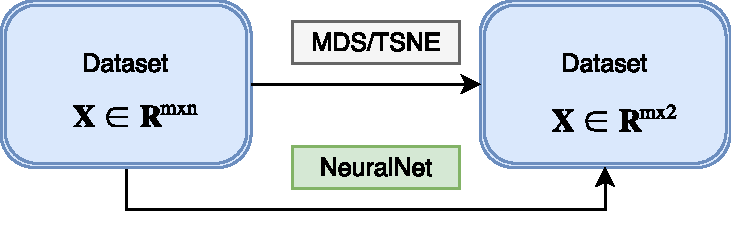
\includegraphics[width=12cm]{figures/neuralnet.pdf}
\caption{\label{figurenet}Dimensionality reduction algorithm learned by a Neural Network}
\end{figure}

\section{Cross Validation}
\label{sec:cv}

Cross validation is a technique to evaluate the predictive models to get to know if the model is capturing the general behaviour of the data to suit new examples, and moreover estimate how accurate the model is performing.\\
The easiest way to know whether a model is underfitting or overfitting is dividing the dataset into train datapoints and test datapoints, choosing for example 80\% to train the model and 20\% to test the behaviour with datapoints which have not been used to adjust the model. Although this is a good first approach, we might be fitting our model to the test points without noticing. This means we might be choosing the model's parameters to fit the test set, and still don't capture the general behaviour of the problem.\\
A more accurate approach would be cross validation. It consists on dividing the data into a number of folds usually depending on the dataset. Choosing between three to five folds would be the best decision. The algorithm is then trained the same number of times as folds, choosing in each iteration one of the folds to test and the rest of them to train. As we have trained and tested the model with disjoint values, we are not fitting our model to certain values. We use a losses metric to cuantify this result and to conclude we calculate a mean of all of them to obtain a unique value to represent the total behaviour. A schema is shown below to represent what cross validation is doing.\\

\begin{figure}[h]
\centering
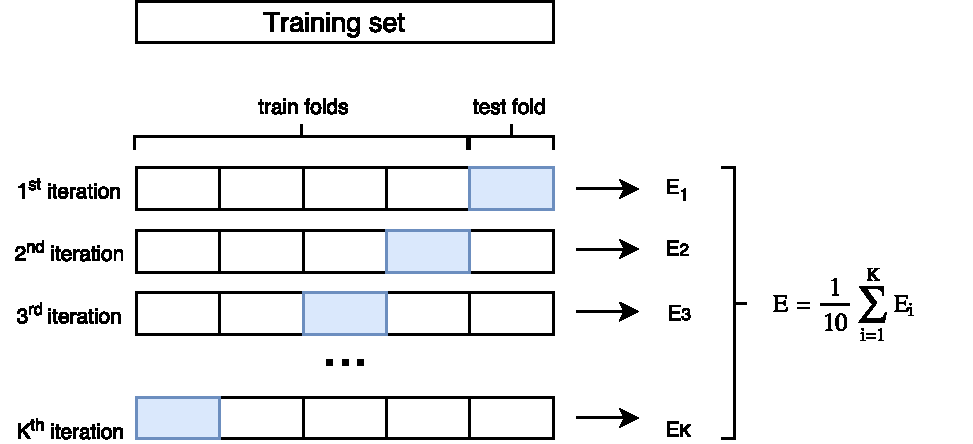
\includegraphics[width=12cm]{figures/cv.pdf}
\caption{\label{figurefit}Cross validation using K-Folds.}
\end{figure}

%-----------------------------------------------------
% Chapter: Applications
%-----------------------------------------------------

\chapter{Applications}
\label{chap:app}

\section{Application 1: Replicating t-SNE with Neuralnet}
\label{sec:app1}

The first implementation to be described is the model which replicates the non-parametric dimensionality reduction algorithm. In this concrete example, T-Stochastic Neighbour Embedding is used as the problem to carry out. The main objective is to assess whether the supervised neuralnet is capable of replicating the previous algorithm.

\subsection{Dataset}
\label{ssec:data1}

The dataset \textit{"load-digits"} is the data used to develop this example and is extracted from the Scikit-Learn datasets \citep{scikit-learn}. It consists on 1797 instances of handwritten digits between 0 to 9 from diferent writers with 64 features each. This features display the values of grayscale intensity for each pixel in the image. This means our images are 8x8 pixel images which are represented by 64 total features containing intensities from 0 (completely black) to 16 (pure white) as show in figure \ref{figuredigit}. To translate this into a dataset, each image is represented in a row with its corresponding 64 values and including a last column with the label of the number represented in the image.
\begin{figure}[h]
\centering
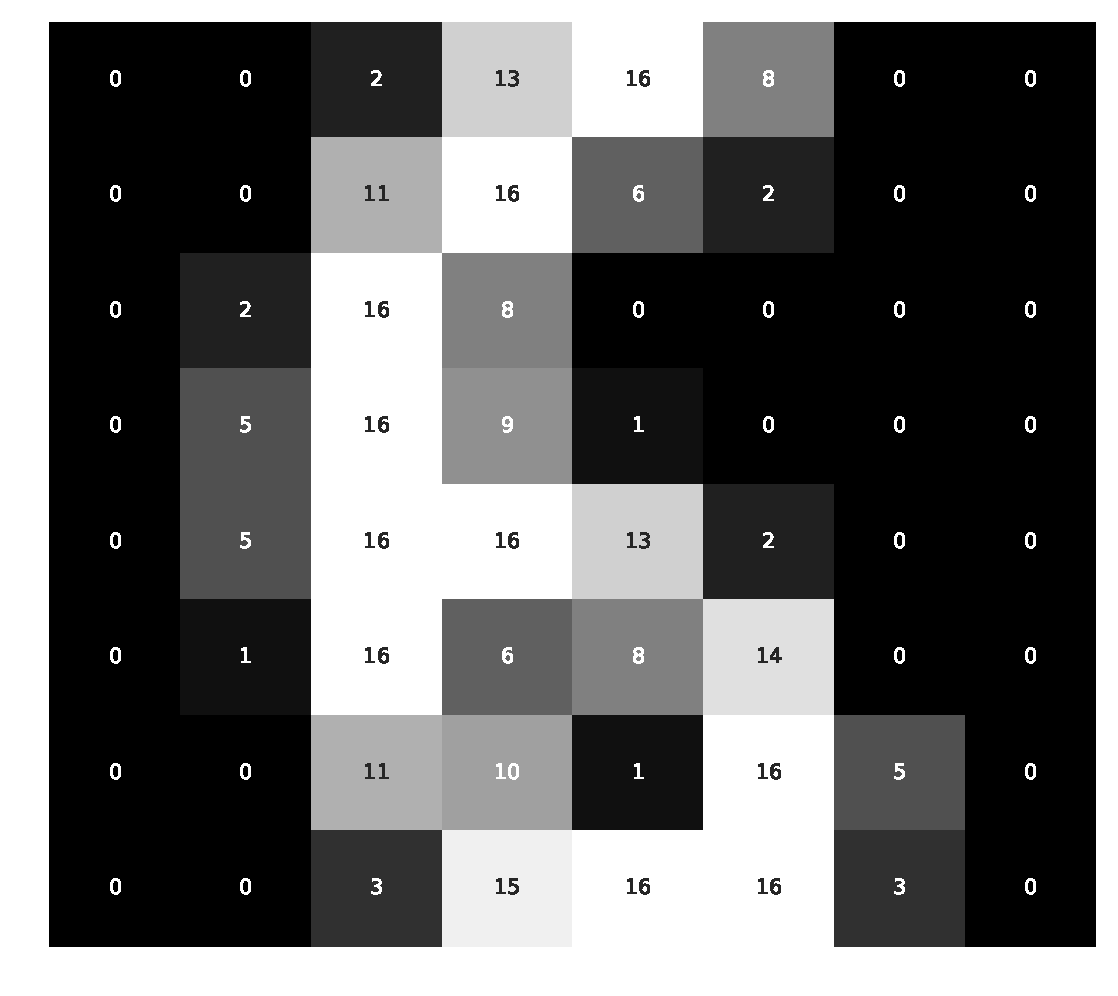
\includegraphics[width=10cm]{figures/exampledigit.pdf}
\caption{\label{figuredigit}Example dataset point representing a handwriten digit.}
\end{figure}

\subsection{Algorithm: t-SNE and Neuralnet}
\label{ssec:dra}

This section comprehends the next points to take into account: the computation of the dimensionality reduction algorithm and its implementation in the neuralnet model.

As a basis to the problem, t-SNE is computed to all the datapoints. Previously, standardizating features in the original data by removing the mean and scaling to unit variance is computed for each of the 64 variables, which achieves better results afterwards. Due to the dataset composed by 1797 instances with 64 features each, a two dimensional space reduction is calculated, looking forward to visualizating the data.

Once reduced data is obtained, both the original and the just calculated points are divided into two corresponding folds, one being a subsample for training the neuralnet and the other to test the model. Therefore, overfitting is avoided by using completely different data to train than to test if the neuralnet is capturing the general behaviour of the dimensionality reduction algorithm.

To continue, the next to keep in mind is the neuralnet's construction. There are several types of neuralnets depending on how it's built, mainly if they are composed by a few layers (1-2 layers) or more layers, and the number of neurons per layer, obtaining shallow or deep and wide or narrow neuralnets correspondingly. Depending on the net computed, the results gathered will differ from one another, thus on section \ref{ssec:met1} the diferences between them are shown.

Once the net is stablished, the standardized original data from the training subsample turns to be the net's input in the fitting process. The output will always be a two variable output, corresponding to the two values which represent the dimension reduction. At this point, the model also uses the training subsample from the reduced points originated in the t-SNE's computation as the output to obtain and to learn from.\\
The neuralnet seeks to get the same output as the dimensionality reduction algorithm, that is why the metric used to minimize the error tends to be a distance metric. It tries to reduce the distance between the values from t-SNE and the values being learned by the model. In this case the distance metric which obtains better results corresponds to the mean of the distances between corresponding points, but other metrics can also be used such as mean loss (mean of the square of the difference between points).

To conclude, as the net has been trained to obtain two output values depending on the 64 feature standardized values in the input, it is possible to predict, taking into account the new input, the reduced data replicating what t-SNE would compute but avoiding the need to recalculate the whole algorithm.\\

\begin{algorithm}
\caption{Neuralnet replicating process}
\begin{algorithmic}[1]
\Procedure{Replicating Procedure}{}
\BState \emph{data obtaining}
\State $\textit{\textbf{X}} \gets \text{standardized input matrix}$
\State $\textit{\textbf{X\_tsne}} \gets \text{compute t-SNE from \textit{\textbf{X}}}$
\State $\textit{\textbf{X\_train; }} \textit{\textbf{X\_test; }} \textit{\textbf{X\_tsne\_train; }} \textit{\textbf{X\_tsne\_test; }}  \gets \text{train and test data computation}$
\BState \emph{neuralnet model construction}
\BState \emph{fit neuralnet model}
\State $\textit{\textbf{X\_train}} \gets \text{neuralnet's input}$
\State $\textit{\textbf{X\_tsne\_train}} \gets \text{neuralnet's output}$
\State $\textit{\textbf{distance error}} \gets \text{neuralnet's error metric}$
\BState \emph{predict neuralnet model}
\State $\textit{64 feature input (new example)} \to \text{neuralnet} \to \text{predict output = } \text{\underline{dimension reduction}}$
\EndProcedure
\end{algorithmic}
\end{algorithm}

\subsection{Metrics}
\label{ssec:met1}

With this first implementation we look forward to obtain reduced data in less computational time using the most accurate neuralnet model depending on its construction. Depending on the type of neuralnet used, times and errors are calculated in the following tables (tables \ref{metrics1} and \ref{times1}).

The most important point by now is that this measurements are done with examples from the test subsample which have not been used by the neuralnet to compute its fitting process, thus they indicate the general behaviour of the model.

Table \ref{metrics1} includes the model construction and the errors computed. The model construction depends on the layers and the number of neurons per layer and on the dropout applied for each layer. Those two values are declared with arrays as in the table is shown. As a resume, the type of the neuralnet built is summarized in deep or shallow and wide or narrow nets.\\
The out of sample error computed is again a distance error which evaluates the difference between what the t-SNE computed and what the model is predicting. The error variable then corresponds to the mean of the Euclidean distances between the two algorithms. Percentages are also included to reckon whether the total error compared to the range of values acquired by the algorithms stand in a good proportion.

\begin{table}[h]
\vspace{20px}
\centering
\begin{tabular}{llllrrr}
\toprule
{} &       dropout &             layers &              type &     error &  \%error\_X &  \%error\_Y \\
\midrule
model1 &  [0, 0, 0, 0] &    [32, 16, 16, 8] &     deep - narrow &  6.335186 &  4.976027 &  5.882600 \\
model2 &        [0, 0] &           [32, 32] &  shallow - narrow &  5.810866 &  4.564196 &  5.395738 \\
model3 &        [0, 0] &           [32, 16] &  shallow - narrow &  6.276359 &  4.929821 &  5.827976 \\
model4 &     [0, 0, 0] &      [128, 64, 64] &       deep - wide &  3.379963 &  2.654821 &  3.138498 \\
model5 &  [0, 0, 0, 0] &  [128, 64, 64, 32] &       deep - wide &  3.481527 &  2.734596 &  3.232807 \\
model6 &     [0, 0, 0] &    [128, 128, 128] &    shallow - wide &  3.239071 &  2.544157 &  3.007672 \\
model7 &        [0, 0] &          [128, 64] &    shallow - wide &  4.151196 &  3.260593 &  3.854634 \\
model8 &           [0] &             [1000] &   shallow - wider &  5.510108 &  4.327962 &  5.116465 \\
\bottomrule
\end{tabular}

\caption{\label{metrics1}Comparison between model's errors obtained out of sample}
\end{table}

Neuralnet's background consists on matrix scalar multiplications of vectors with learnt parameters and activation functions, hyperbolic tangent in this problem, which are very efficient computationally operations.\\
Table \ref{times1} shows the huge difference between the computational time (in seconds) of the dimensionality reduction algorithm and the neuralnet's development for the same number of points, refering to the whole dataset (1787 points in total).

\begin{table}[h]
\vspace{10px}
\centering
\begin{tabular}{lr}
\toprule
{} &      times \\
\midrule
tsne   &  49.129993 \\
model1 &   0.132459 \\
model2 &   0.111072 \\
model3 &   0.130287 \\
model4 &   0.175929 \\
model5 &   0.190567 \\
model6 &   0.227528 \\
model7 &   0.211757 \\
model8 &   0.252915 \\
\bottomrule
\end{tabular}

\caption{\label{times1}Computational times}
\end{table}

\subsection{Conclusion}
\label{ssec:conc1}

Consequently and given the results in the previous tables, we can reassure that, without considerating the neuralnet's construction, all of them will certainly be quicker in obtaining the results. If we look for accuracy, a wide neuralnet is better at replicating the t-SNE algorithm. In particular, the model 6 proposed suits the best for the problem presented.\\
The next two figures represent the results obtained. The first one matches the predictions from the neural network (in model 6) and the second one represents the same points from the t-SNE algorithm.

\begin{figure}[p]
\centering
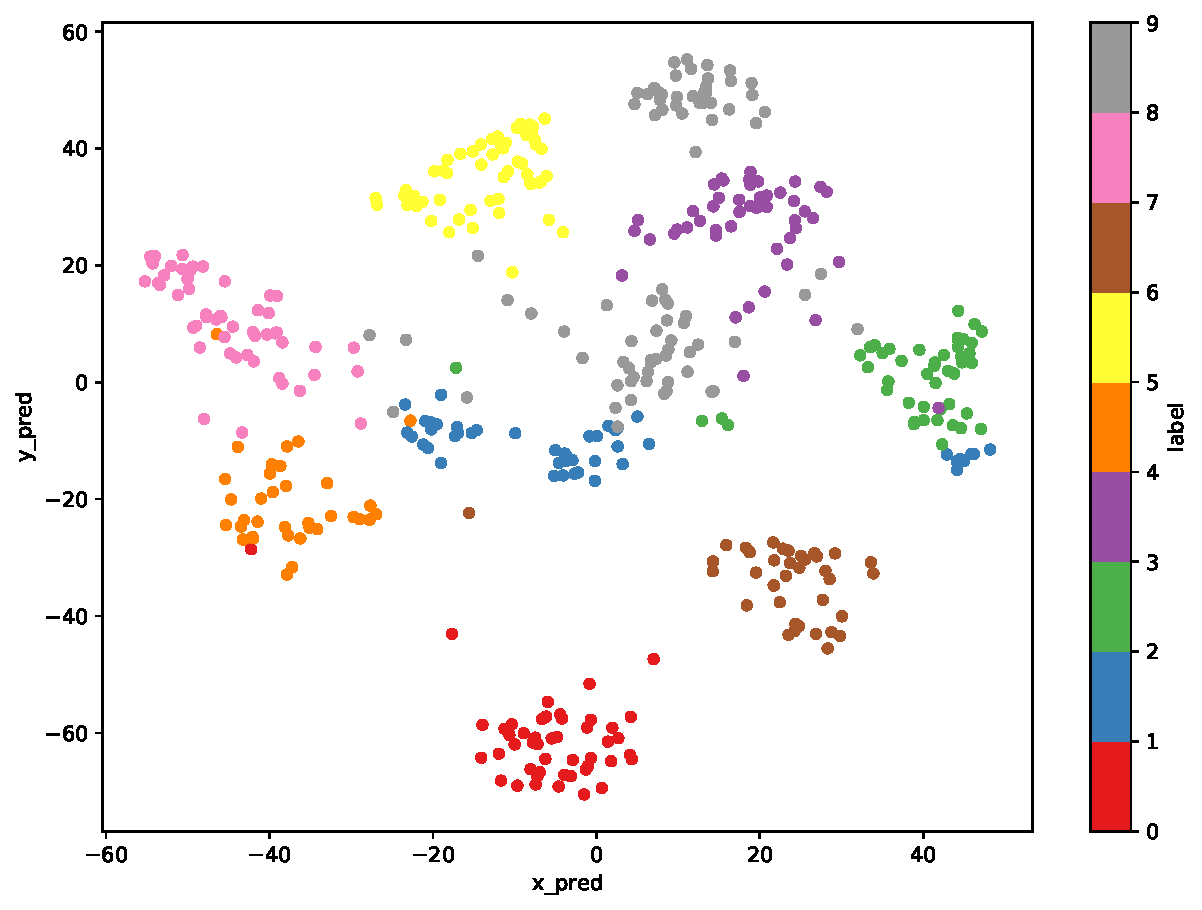
\includegraphics[width=12cm]{figures/app1plotpredictions.pdf}
\caption{\label{figureNN}Low dimensional space from NeuralNet.}
\end{figure}

\begin{figure}[p]
\centering
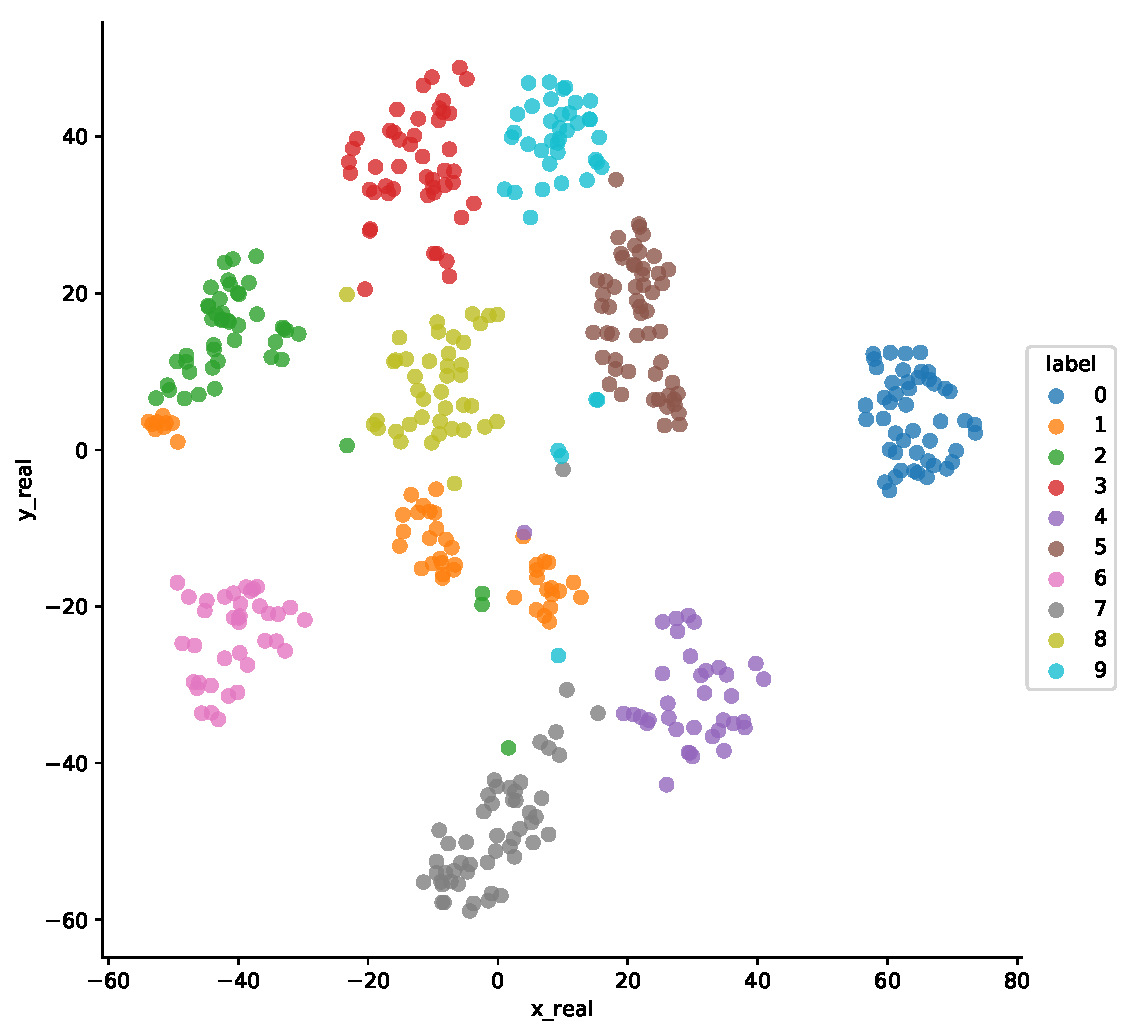
\includegraphics[width=12cm]{figures/app1plotreal.pdf}
\caption{\label{figureTSNE}Low dimensional space from from t-SNE}
\end{figure}

\newpage

\section{Application 2: Nearest Neighbours calculation}
\label{sec:app2}

The second application consists on the computation of nearest neighbours in a low-dimensional space. This second implementation focuses on the Multidimensional Scaling algorithm. The aim is to compute the nearest neighbours in the output coordinates from MDS. A loss in precision and recall is involved in the nearest neighbours computation since an error in computation is made when calculating the low dimensional equivalent points. Nevertheless, it allows for a faster, low memory intensive algorithm.

\subsection{Dataset}
\label{ssec:data2}

The dataset \textit{"forests.csv"} is used for this application and is extracted from UCI Machine Learning Repository \citep{ucidata}. For convenience, a random subsample of 20.000 examples is storaged with 55 features each. These are all numeric variables that describe several characteristics of the forest. The forest type output is represented by a number in range 1 to 7, shaping the last column of the dataset.\\
The reason why this dataset is chosen for this concrete application relies on the need to compute a substantial amount of examples in the training phase to obtain a reliable model and to be able to asses time and memory performance improvements and also recall/precision degradation.

\subsection{Algorithm: Low dimensional nearest neighbors obtaining}
\label{ssec:nneigh}

The main task contemplated in this application is the computation of nearest neighbours. The following research bears with reusability and time and memory usage reduction algorithms.

Regarding the first point, because of MDS being non-parametric, it is uncapable of obtaining new embedded points without computing again all the operations. This means if we have already output the low-dimensional map of points from the dataset, it would not be posible to obtain a new point in this map unless the algorithm is recomputed. If we based our nearest neighbours search in a previous dimensionality reduction algorithm such as MDS, the only results available would be from the points just computed by MDS.

Nearest neighbours brute force models \citep{brute} are known to be eficiently poor when a raw dataset is provided, both because their memory tends to be big and thus the computational time required also increases.\\
Nearest neighbours brute force algorithm computes the euclidean distances between each point and the rest of the data and then sortens them according to their distances, from lowest to highest, for each of the examples in the dataset. This means the computational complexity corresponds to $O(n^{2})$. Since the euclidean distances is computed as:
$$ dist(p,q) = \sqrt{(q_{1}-p_{1})^{2}+(q_{2}-p_{2})^{2}+ ... + (q_{n}-p_{n})^{2}} = \sqrt{\sum_{i=1}^{n} (q_{i}-p_{i})^{2}}$$
The brute force algorithm's complexity in terms of dimensions computed, d, is $O(n^{2}*d)$.\\
As for the memory and taking into account the previous ideas of how to compute neighbours, this model requires the original matrix to be stored which means the memory complexity also depends on the number of points and their dimensions and is resumed in a $O(n*d)$ model.

The next model is a new solution proposed to solve the problems just mentioned.\\
The algorithm involves two phases: one fitting process and its later usage for new points. This is why the original dataset is splitted into two folds, one for the training and the second one to test out of sample performance.

The training phase aims to obtain all the parameters or transformations which will be later used to transform the data. During the fitting process, the MDS computes the embeddings (vectors of all samples in the embedding space) directly by using gradient descent on its loss function (stress). This is why we would not be able to obtain the tranformation of a new sample without having to fit the whole dataset again (which requires computational time), thus we would not be able to step into the process of computing nearest neighbours in the low-dimensional space.\\
Instead, in this proposal, and as seen in the first application (\ref{sec:app1}), the training consists on faithfully learning the mapping of a dimensionality reduction algorithm from a high-dimensional space to a low-dimensional space by training a neuralnet to do so. In this case, the model saves the neuralnet's parameters which replicate the MDS, instead of the exact transformations from it. Then, when a new out of sample point is included, there is no need to compute the whole MDS algorithm to be able to transform the data because we have a neuralnet that can approximate the embedding operation.\\
Accordingly, the approximate nearest neighbours model designed will have its computational time and memory complexity reduced by the relation between the original (\textit{d}) and the low-dimensional space's dimensions (\textit{k}).
\begin{itemize}
\item Computational time complexity: $O(N^{2}*K)$
\item Memory complexity: $O(N*K)$
\end{itemize}

To conclude, when a new sample is requested to find the k-nearest neighbours, it is firstly transformed by the neural net from \textit{d} dimensions to \textit{k}, corresponding to the low-dimensional space, by predicting with the embedding learnt from MDS. Afterwards, the nearest neighbours are computed comparing the new example with the rest of the low  dimensional samples, achieving a faster and low memory intensive algorithm.\\

\begin{algorithm}
\caption{Low dimensional nearest neighbours calculation}
\begin{algorithmic}[1]
\Procedure{Fitting process}{}
\State $\textit{\textbf{X}} \gets \text{imputed and standardized dataset}$
\State $\textit{\textbf{X\_mds}} \gets \text{compute MDS from \textit{\textbf{X}}}$
\BState \emph{neuralnet model construction}
\BState \emph{fit neural net model}
\BState \emph{save reduced matrix from training neural net}
\EndProcedure
\end{algorithmic}
\end{algorithm}
\hfill

\begin{algorithm}
\caption{Low dimensional nearest neighbours calculation}
\begin{algorithmic}[1]
\Procedure{NN calculation for new sample}{}
\State $\textit{\textbf{x}} \gets \text{new sample}$
\State $\textit{\textbf{x\_reduced}} \gets \text{predicted output from neural net with x (reduction)}$
\BState \emph{nearest neighbours calculation with brute force algorithm in the low dimensional space}
\EndProcedure
\end{algorithmic}
\end{algorithm}

\subsection{Metrics}
\label{ssec:met2}

With this second implementation, the main metrics to look at correspond to precision and computational measurements, such as time and memory usage. As the objective is to finally compute nearest neighbours, precision is described as the percentage of nearest neighbours preserved in comparison to bruce force algorithm. In the case of time and memory, the measurements are strictly related to the algorithm's performance, thus we calculate how much time they require to compute the neighbours and the memory the data needs to do so.

The following tables relate the model used to compute the neural net with the previous metrics, depending on the dimensions of the low-dimensional space chosen to lower the data's features.

\begin{table}[p]
\centering
\begin{tabular}{lrrrrr}
\toprule
{} &  \ npreserved &    t\_model &  t\_brute &  mem\_model &  mem\_brute \\
\midrule
model1 &     0.565350 &  0.771945 &  1.074873 &     112112 &   3080112 \\
model2 &     0.571843 &  0.785027 &  1.084613 &     112112 &   3080112 \\
model3 &     0.570347 &  0.800511 &  1.067814 &     112112 &   3080112 \\
model4 &     0.567003 &  0.755689 &  1.082235 &     112112 &   3080112 \\
model5 &     0.564130 &  0.796335 &  1.038609 &     112112 &   3080112 \\
model6 &     0.564723 &  0.808626 &  1.021288 &     112112 &   3080112 \\
model7 &     0.569093 &  0.767841 &  1.096126 &     112112 &   3080112 \\
model8 &     0.572430 &  0.922942 &  0.888819 &     112112 &   3080112 \\
\bottomrule
\end{tabular}

\caption{\label{metrics21}Nearest neighbours calculation in four dimensions}
\end{table}

\begin{table}[p]
\centering
\begin{tabular}{lrrrrr}
\toprule
{} &  \%npreserved &    nntime &  realtime &  mem\_model &  mem\_real \\
\midrule
model1 &     0.728400 &  0.993689 &  1.204910 &     224112 &   3080112 \\
model2 &     0.780377 &  0.969519 &  1.218967 &     224112 &   3080112 \\
model3 &     0.779553 &  0.971488 &  1.219617 &     224112 &   3080112 \\
model4 &     0.760667 &  0.974497 &  1.152932 &     224112 &   3080112 \\
model5 &     0.761370 &  0.978987 &  1.146578 &     224112 &   3080112 \\
model6 &     0.756977 &  0.990972 &  1.081272 &     224112 &   3080112 \\
model7 &     0.771057 &  0.972610 &  1.216437 &     224112 &   3080112 \\
model8 &     0.771207 &  1.006541 &  0.947692 &     224112 &   3080112 \\
\bottomrule
\end{tabular}

\caption{\label{metrics22}Nearest neighbours calculation in eight dimensions}
\end{table}

\begin{table}[p]
\centering
\begin{tabular}{lrrrrr}
\toprule
{} &  \ npreserved &    nntime &  realtime &  mem\_model &  mem\_real \\
\midrule
model1 &     0.669377 &  0.952179 &  1.175327 &     504112 &   3080112 \\
model2 &     0.855583 &  0.953779 &  1.175554 &     504112 &   3080112 \\
model3 &     0.837507 &  0.950562 &  1.197267 &     504112 &   3080112 \\
model4 &     0.848860 &  0.961237 &  1.126327 &     504112 &   3080112 \\
model5 &     0.844383 &  0.955949 &  1.114451 &     504112 &   3080112 \\
model6 &     0.835173 &  0.966225 &  1.045986 &     504112 &   3080112 \\
model7 &     0.855930 &  0.955785 &  1.174047 &     504112 &   3080112 \\
model8 &     0.853597 &  0.945284 &  0.928504 &     504112 &   3080112 \\
\bottomrule
\end{tabular}

\caption{\label{metrics23}Nearest neighbours calculation in eighteen dimensions}
\end{table}

The approximate model designed can also be compared to other approximate nearest neighbours algorithms such as KD-Tree \citep{kdtree}. KD-Tree is a binary tree that represents a division of the space using splitting planes which are orthogonal to the axis. Each node has a corresponding region called cell and the root's cell has to include all the points from the dataset. For each region we have a hyperplane which divides the points into one side or the other, until there are no points left, which means the partition is over and the tree is constructed. This type of tree achieves a computational complexity of $O(NlogN)$ and works correctly for low-dimensional datasets. When the dimensions get higher, the behaviour tends to get worse. Table \ref{metrics24} corresponds to the first dataset of the application.

\begin{table}[h]
\centering
\begin{tabular}{lrrrrr}
\toprule
{} &  \%npreserved &    nntime &  realtime &  mem\_model &  mem\_real \\
\midrule
model1 &          1.0 &  2.599825 &  1.173718 &    3080112 &   3080112 \\
model2 &          1.0 &  2.633631 &  1.157942 &    3080112 &   3080112 \\
model3 &          1.0 &  2.624684 &  1.168484 &    3080112 &   3080112 \\
model4 &          1.0 &  2.613410 &  1.153366 &    3080112 &   3080112 \\
model5 &          1.0 &  2.614144 &  1.169271 &    3080112 &   3080112 \\
model6 &          1.0 &  2.609788 &  1.184947 &    3080112 &   3080112 \\
model7 &          1.0 &  2.637135 &  1.164681 &    3080112 &   3080112 \\
model8 &          1.0 &  2.612835 &  1.174181 &    3080112 &   3080112 \\
\bottomrule
\end{tabular}

\caption{\label{metrics24}KD-Tree computing nearest neighbours}
\end{table}

Although the total of neighbours are preserved, both the computational time and memory the model consume are high, two times compared to brute force algorithm. This means that if a bigger dimensional dataset or more intances are provided, the algorithm tends to be non-scalable, thus the capacity of the algorithm in terms of computational time and memory turns the model into a complex one.\\
To prove this, the next to tables compare the approximate model and the kd-tree approximate nearest neighbours computation with a new dataset that has 4000 instances and 281 features per sample.

\begin{table}[h]
\centering
\begin{tabular}{lrrrrr}
\toprule
{} &  npreserved &   t\_model &   t\_brute &  mem\_model &  mem\_brute \\
\midrule
model1 &     0.30045 &  0.152567 &  0.206344 &    1200112 &    6744112 \\
model2 &     0.43732 &  0.140289 &  0.172093 &    1200112 &    6744112 \\
model3 &     0.38892 &  0.139835 &  0.178780 &    1200112 &    6744112 \\
model4 &     0.46497 &  0.132087 &  0.177754 &    1200112 &    6744112 \\
model5 &     0.41835 &  0.132285 &  0.173796 &    1200112 &    6744112 \\
model6 &     0.49443 &  0.133642 &  0.174198 &    1200112 &    6744112 \\
model7 &     0.50684 &  0.136121 &  0.174210 &    1200112 &    6744112 \\
model8 &     0.59107 &  0.136980 &  0.184086 &    1200112 &    6744112 \\
\bottomrule
\end{tabular}

\caption{\label{metrics25}Nearest neighbours calculation in 100 dimensions from new dataset}
\end{table}

\begin{table}[h]
\centering
\begin{tabular}{lrrrrr}
\toprule
{} &  npreserved &   t\_kdtree &   t\_brute &  mem\_kdtree &  mem\_brute \\
\midrule
model1 &     0.99992 &  2.211247 &  0.383505 &   13808037 &    6744112 \\
model2 &     0.99992 &  2.088237 &  0.442901 &   13808037 &    6744112 \\
model3 &     0.99992 &  1.973441 &  0.446145 &   13808037 &    6744112 \\
model4 &     0.99992 &  1.844881 &  0.388873 &   13808037 &    6744112 \\
model5 &     0.99992 &  2.136054 &  0.422400 &   13808037 &    6744112 \\
model6 &     0.99992 &  1.878483 &  0.433052 &   13808037 &    6744112 \\
model7 &     0.99992 &  2.173580 &  0.405178 &   13808037 &    6744112 \\
model8 &     0.99992 &  1.897629 &  0.438579 &   13808037 &    6744112 \\
\bottomrule
\end{tabular}

\caption{\label{metrics24}KD-Tree computing nearest neighbours from new dataset}
\end{table}

The computational time KD-Tree requires is twelve times the computational time from the approximate model in the best of the cases. The memory KD-Tree needs to compute its operations is nearly also twelve times in comparison to the model designed in this dataset.

\subsection{Conclusion}
\label{ssec:conc2}

Computing nearest neighbours in nowadays applications has become an important topic. The need to report them quickly demands new algorithms like the model previously designed. It consists on lowering the sample's dimensions with a neural net which has learnt how to do it by replicating a MDS, and then, nearest neighbours are computed in the low-dimensional space.\\
As seen in the results studied before, there is a relation between precision obtained and time and memory usage.\\
Although KD-Tree also uses the idea of lowering the data's features, regarding precision, time and memory usage this gets higher when a complex dataset is provided.\\
With this model we obtain less precision by computing rapidly and with less memory usage.

The computational complexities for the three algorithms studied are the next ones (taking into account dimensions computed):
\begin{itemize}
\item Brute force algorithm: $ O(N^{2}*D)$ 
\item KD-Tree algorithm: $ O(NlogN*D)$ 
\item Approximate nearest neighbours algorithm: $ O(N^{2}*D^{*}) = O(N^{2}*\frac{D}{3})$ 
\end{itemize}

The following figure describes this computational complexities for a given number of dimensions:

\begin{figure}[h]
\centering
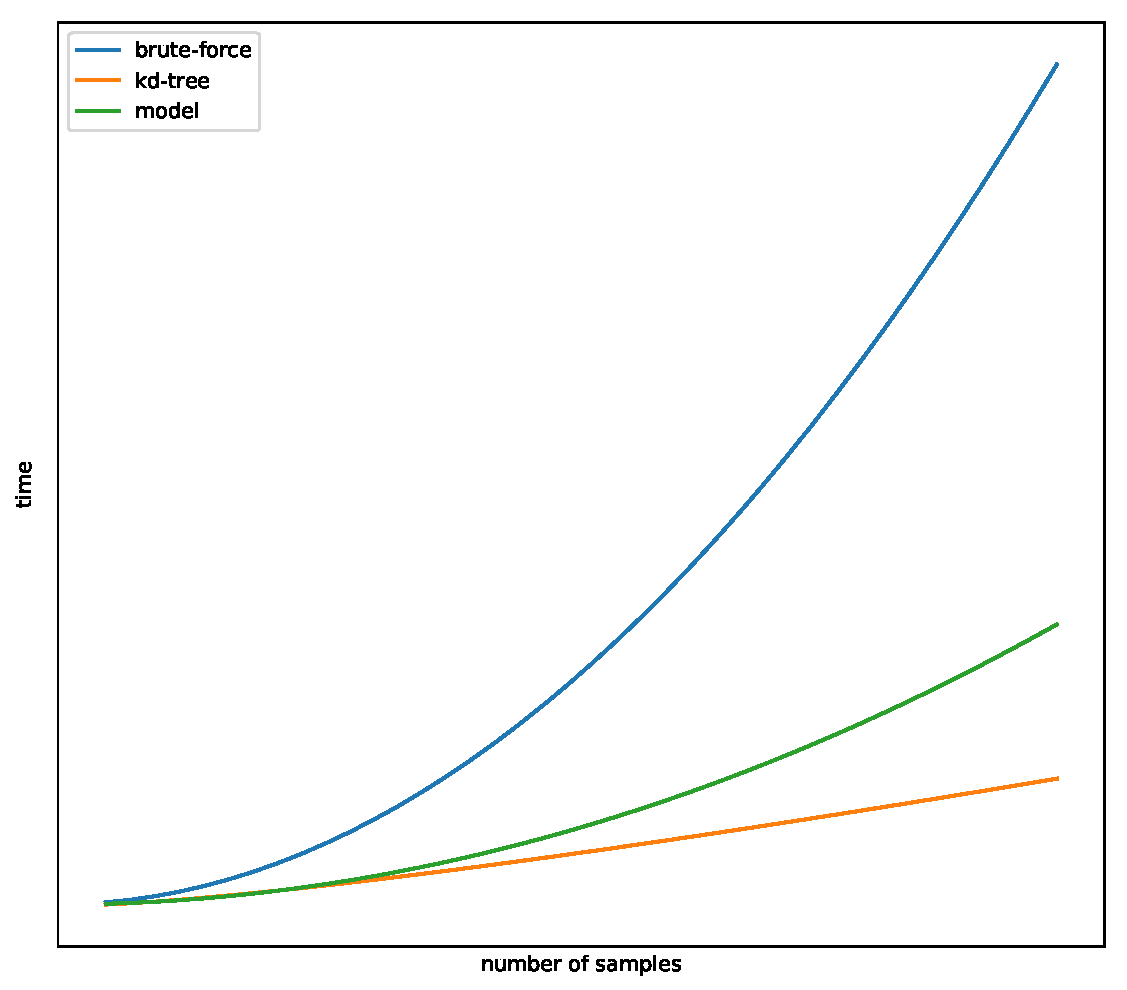
\includegraphics[width=12cm]{figures/complexities.pdf}
\caption{\label{figureNN}Algorithms' complexities.}
\end{figure}


%%%%%%%%%%%%%%%%%%%%%%%%%%%%%%%%%%%%%%%%%%%%%%%%%%%%%%%%%%%%%%%%
%%%% previous work, not important yet
\newpage

We have developed a supervised algorithm, based in neuralnets, which reproduces the ideas showed in the framework's introduction.
The inputs expected to run this algorithm are the next ones:

\begin{itemize}
\item Number of components for the low-dimensional space
\item Dimensionality reduction object, such as PCA, MDS or TSNE in our examples.
\item Layers: the number of layers and neurons per layer, taking into account that the last layer has the same neurons as the number of components in the low dimensional space; e.g: layers = 2; neurons = 100, 10; it has three layers, with 100, 10 and the number of components neurons each.
\item Dropouts: percentage of neurons from each layer used for training.
\item Learning rate for the neural network training.
\item Activation function for the neuralnet.
\item Losses function used to minimize the cost.
\item Number of epochs for each training, being epochs the number of times the whole training set has been passed through the neuralnet.
\item Batch size: number of examples used to compute the gradient of the cost function.
\end{itemize}

The future sections \ref{ssec:nnc}, \ref{ssec:fit} and \ref{ssec:trans} resume some more ideas about the supervised algorithm, describing the construction of the neuralnet, the fitting process and the dimensionality reduced data obtaining.

\subsection{Neuralnet construction.}
\label{ssec:nnc}

This function is in charge of constructing the neural network taking into account the inputs provided. A neuralnet is defined by the number of layers, number of neurons per layer, activation function, dropouts and loss function. To train the neuralnet we need to specify the number of epochs and batch size.

\subsection{Fitting process.}
\label{ssec:fit}

The fitting process seeks the parameters or values obtained from a training process given a specific dataset. Depending on whether it is a supervised or non-supervised algorithm, the output of this operations will be either some parameters or directly the remodeled values. For example, as PCA is a parametric transformation, fitting will determine the dimensionality reduction matrix which could afterwards be used to determine the modified data. On the other hand, MDS and TSNE are non-parametric dimensionality reduction algorithms, so the fitting process directly obtains the values from the lower dimension. This parameters and values in the fitting process are stored as an object's own variable until necessary.

We look forward to construct a supervised learning algorithm, based on neuralnets, and we want to obtain the parameters learning from the unsupervised embedding algorithm. The steps to take would be as follows: firstly comes the construction of the neuralnet, taking into account what was said in the previous section plus the input matrix's input. Second of all, we have to store the reduced data from the embedder algorithm. At last, we have the original data and the reduced computed data, so we decided to fit the neuralnet with both datasets and store the output parameters of the neuralnet.
\vspace{10pt}


We have been able to turn a unsupervised learning algorithm into a supervised learning algorithm, by replicating the unsupervised algorithm's behaviour.

\subsection{Dimensionality reduced data obtaining.}
\label{ssec:trans}

We have achieved the task of replicating an unsupervised algorithm's behaviour by a supervised algorithm, characterized for being capable of predicting the output by computing operations between the input and some learned parameters.
Even though the unsupervised algorithms have no parameters, a neuralnet does. We have obtained, using those parameters, prediction outputs from the new datapoints, which copy the dimensionality reduction without the need to compute the whole algorithm.



%-----------------------------------------------------
% Chapter: Conclusion
%-----------------------------------------------------

\chapter{Conclusion}
\label{chap:conc}


%-----------------------------------------------------
% Chapter: Extra
%-----------------------------------------------------

\chapter{EXTRA APPENDIX}
\label{chap:append}

We have developed a class named NNReplicator which replicates the behaviour of a neuralnet wrapping an embedder object, as it is represented in figure \ref{figurenet}. It is written as if it was a Scikit Learn class so that the objects created could fix into a Scikit Learn pipeline, being one of the main future applications.

Once the inputs are understood, the next point is to get to know what is being computed and what methods are included in the class. As we want to include it as a Scikit Learn class, some methods are required; those are the methods fit and transform, which make the class capable of instantiate tranformers, objects that vary the data input into some output.

It is based on the Keras library, which makes easier the task of programming a neuralnet. A sequential model is used to stack one layer after the other. We use: add Dense to include a layer, add Activation to specify which activation function to use and add Dropout to include the porcentage of dropout indicated by the corresponding input.\\
The best way of implementing the neural net is by designing a for-loop which extracts the inputs from the arrays and automatically computes denses and dropouts.\\
The default optimizer is Adagrad, and takes as input the learning rate from the object's inicialization. The next step should be the compilation of the whole neural net, using the loss function inputed as the cost to minimize and the model should be completely done.\\
Despite of having built the neural net correctly, we also need to make it compatible with Scikit Learn. That's why the last step consists on a Keras Wrapper, named Keras Regressor, remodeling the model into a sklearn neuralnet model.

%-----------------------------------------------------
% Chapter: Bibliography
%-----------------------------------------------------

\label{chap:bib}
\addcontentsline{toc}{chapter}{Bibliography}
\bibliography{mybib}
\nocite{*}

% %%%%%%%%%%%%%%%%%%%%%%%%%%%%
% % BIBLIOGRAPHY
% \clearpage
% \phantomsection
% \addcontentsline{toc}{chapter}{Bibliography}
% \bibliography{bib}
% %%%%%%%%%%%%%%%%%%%%%%%%%%%%

%-----------------------------------------------------
% Appendix: Code
%-----------------------------------------------------

\chapter*{Code}
\label{chap:code}
\addcontentsline{toc}{chapter}{Code}

%\begin{tiny}
%\inputminted[baselinestretch=0.5, breaklines]{python}{code.py}
%\end{tiny}

%%%%%%%%%%%%%%%%%%%%%%%%%%%%
% END DOCUMENT
\end{document}
%%%%%%%%%%%%%%%%%%%%%%%%%%%%
